
\subsubsection{Polycrystalline Metals}

With the HCl vapor treatment added to the procedure, temperature-varying gallium contact angle measurements in an argon environment were executed in the aluminum chamber on multiple metal substrates. Polycrystalline samples of high purity ($>$99.99\%) tin, copper, and iron were polished and had liquid gallium deposited on their surfaces. The temperature in the chamber was slowly ($<$10\degree C/min) increased from ~30\degree C to just below 100\degree C. Beyond 100\degree C, the heating tape becomes inconsistent with the intervals of heat applied to the chamber. Photographs of gallium drop profiles are taken at ~10\degree C intervals to observe progression of the drop shape as temperature increases. The same procedure is done as the temperature is decreased to 30\degree C to observe reversibility of this process, since we assume that the thermal expansion of the substrate drives the change in \gamSL from Equation \ref{youngs-eqn-ga}. 

A chemical vapor etch is used to replace the gallium oxide () layer with a gallium chloride layer, restoring the droplet surface tension to nearly that of pure Ga, as shown by Kim \etal To execute the vapor etch, a sessile drop of gallium was formed on the desired surface and a pipette of 37wt\% HCl was brought within 2 cm to etch away the gallium oxide layer. 

It is known that liquid gallium tends to corrode most metal surfaces.\cite{Lewandowski2015,Narh1998,Fitzgerald1999} Since experiments lasted for less than one hour, corrosion between the two metals should not be significant enough to effect the measurement. Later in this \hyperlink{xps-gallium}{section}, the surface stoichiometry effects of the liquid Ga droplet on Galfenol for varying temperatures is examined using X-ray photoelectron spectroscopy (XPS). For the polycrystalline tin and copper samples, gallium began to visibly corrode through the surface between 60\degree C and 70\degree C, as evident by a rapid contact angle decrease on only side of the drop profile, as seen in Figure \ref{fig:copper-tin-gallium-CA}. Polycrystalline iron samples did not experience corrosion problems throughout the experiments. It is expected that as the temperature increases, the thermal expansion of the solid will isotropically expand the drop thus decreasing the contact angle. Some gallium contact angles decrease on iron, but it is often that the decrease occurs on one side of the drop profile as the temperature increases. This is most likely due to the polycrystalline grains having different thermal expansions, hence the drop spreading is anisotropic. This suggests that a single-crystal grain or highly-textured surface grain is needed to properly observe an isotropic drop expansion. 
\begin{figure}
	\centering
	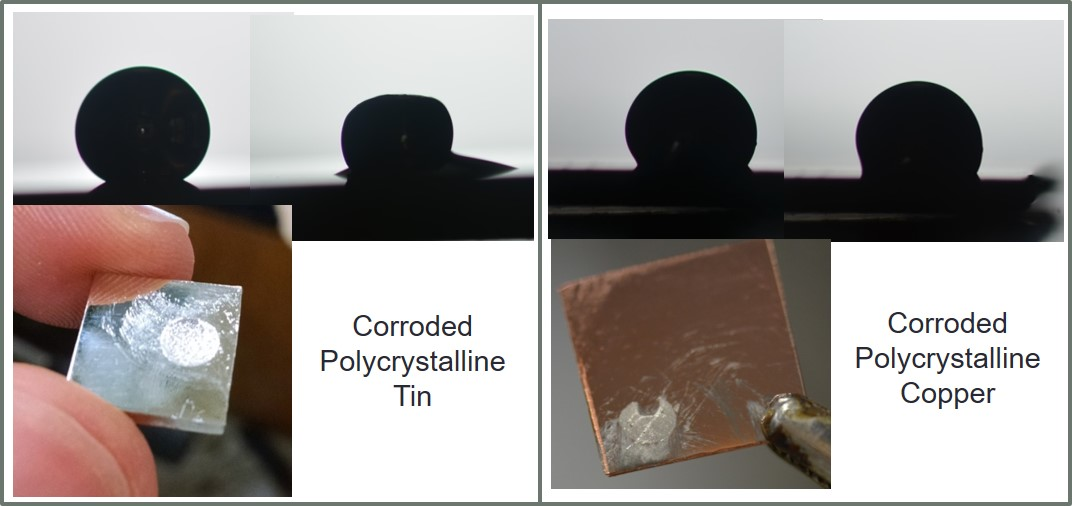
\includegraphics[width=\linewidth,trim={0 0 0 2cm}]{copper-tin-gallium-CA}
	\caption{These photographs show a gallium drop contact angle on polycrystalline Sn (left) and polycrystalline Cu (right), and the corrosive effects of the gallium on the same substrates.}
	\label{fig:copper-tin-gallium-CA}
\end{figure}



Since the iron sample did not corrode in the presence of gallium, we proceeded to a Galfenol sample with an abnormally grown \hkl(110) grain. Figure \ref{fig:ca_ebsd} shows the location of a gallium droplet in contact with the highly Goss-textured surface. Using the same temperature intervals, the right and left contact angles were measured and the surface energy
\begin{figure}
	\centering
	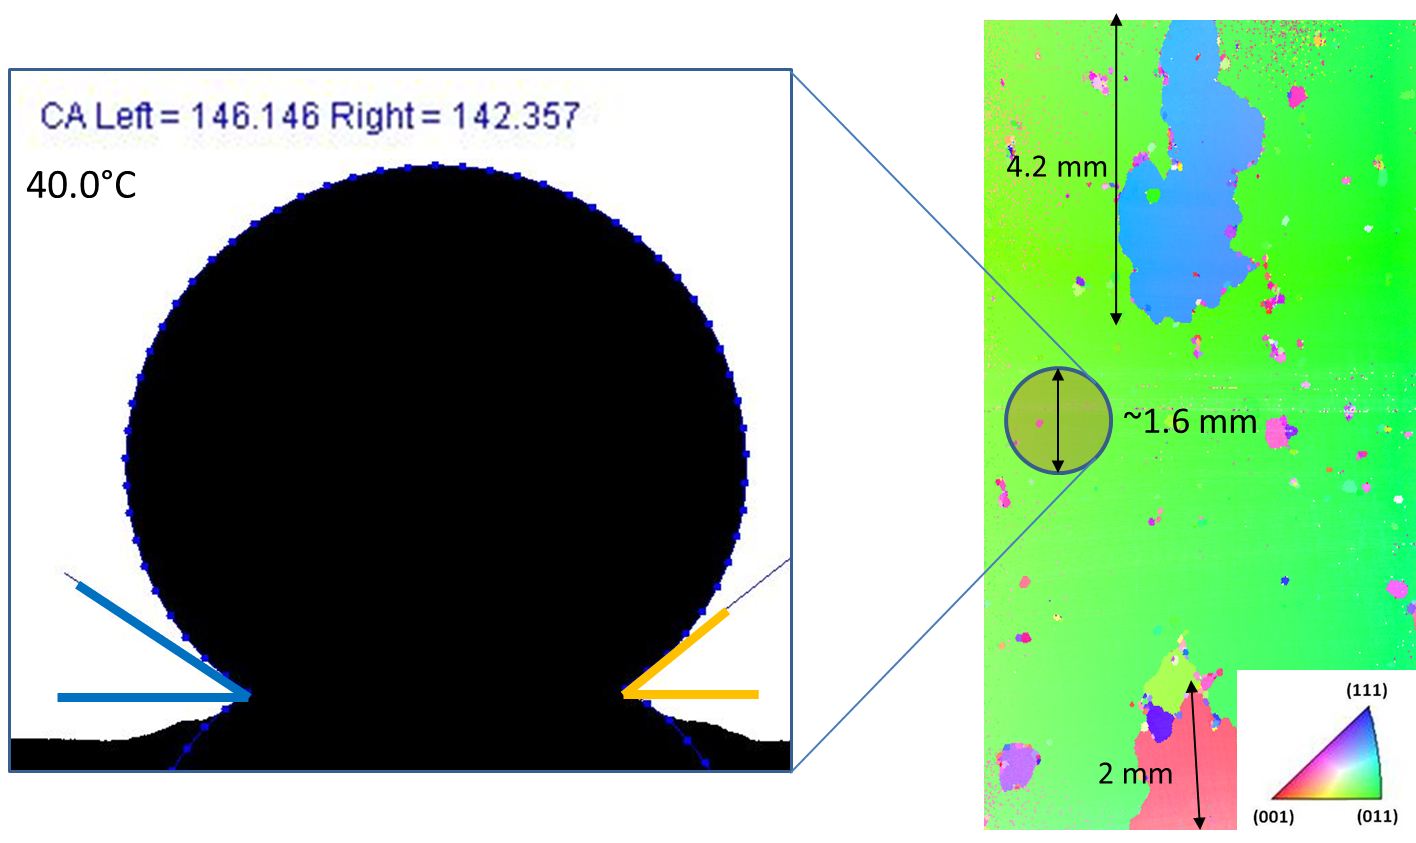
\includegraphics[width=\linewidth,trim={0 0 0 2cm}]{ca_ebsd}
	\caption{The location of a gallium drop on highly Goss-textured surface.}
	\label{fig:ca_ebsd}
\end{figure}
was calculated using Equation \ref{youngs-eqn-ga}. The contact angle measurements and surface energy calculations are shown in Figure \ref{fig:goss_se_msrmnt}. The contact angle measurements show anisotropic spreading behavior since the left contact angle recedes as temperature increases while the right contact angle advances. At 60.7\degree C, the contact angles reached close to the same value which may indicate an equilibrium point of combating thermal expansions caused by nearby island grains. 

Both right and left contact angles were measured at each temperature and used in Equation \ref{youngs-eqn-ga} to calculate the substrate surface energy. Plots of contact angle measurements and surface energy estimates are shown in Figure \ref{fig:goss_se_msrmnt}. The contact angle measurements show anisotropic spreading behavior since the left contact angle recedes as temperature increases while the right contact angle advances. Asymmetries may be associated with nearby island grains that are evident in the electron backscatter diffraction (EBSD) scan of Figure \ref{fig:ca_ebsd}. The magnitude of surface energy values in Figure \ref{fig:goss_ga_se} are on the order of 100 J/m$^2$ and the values increase as temperature increases. We had expected surface energy values to be closer in magnitude to DFT predicted values for $\alpha$-iron of $ \gamma_{SV}(T)$ = 2.0535 J/m$^2$, which has the same body-centered cubic crystal structure as Galfenol.\cite{Wang2000} We had also expected a decrease in surface energy with increasing temperature. This is because surface energy depends on the net inward cohesive force between atoms, and the cohesive force binding atoms to one another will decrease as a temperature increase causes atoms to vibrate more rapidly. We do not yet understand why the model leads to unexpected trends. We are currently examining the role of the $\gamma_{SL}(T)$ term in the model, as it is three orders of magnitude larger than the $\gamma_{SV}(T)$ term (due to the contribution from the Young's modulus value associated with Galfenol) and dominates the results.

\begin{figure}[h]
	\centering
	\begin{subfigure}[c]{0.47\textwidth}
		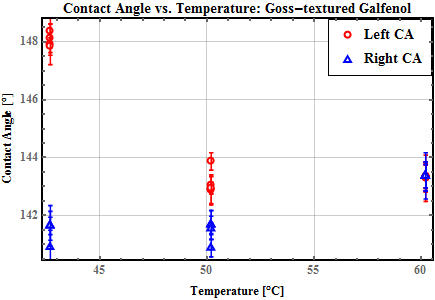
\includegraphics[width=\linewidth]{CAvsTemp_Goss-Galfenol3}
		\subcaption{~}
		\label{fig:goss_ga_ca}		
	\end{subfigure}
	\begin{subfigure}[c]{0.47\textwidth} 
		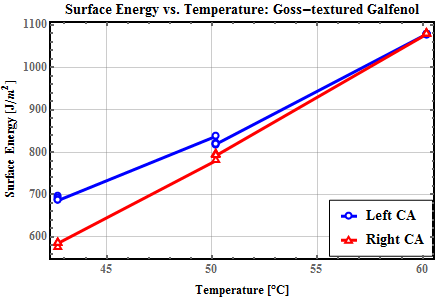
\includegraphics[width=\linewidth]{SEvsTemp_Goss-Galfenol3}
		\subcaption{~}
		\label{fig:goss_ga_se}		
	\end{subfigure}
	\caption{(a) Blue and red dots show left and right contact angle, respectively, of liquid gallium on \hkl(110) Fe-Ga. (b) Calculated surface energy values of \hkl(110) Fe-Ga grains using Equation \ref{youngs-eqn-ga}.}
	\label{fig:goss_se_msrmnt}
\end{figure}





\subsubsection{Single-crystal Galfenol}
Using the same acid vapor etch, Ga droplets were placed on samples of single crystal Galfenol. Contact angle values decrease from the (110), (100), and (111) facets (Figure 4), in that order, although the angles for the (100) and (111) facets are not statistically different (within one standard deviation of one another). According to Young’s equation, these contact angles should be inversely proportional to surface energy. The measurements indicate that the surface energy of a (110) surface has the lowest surface energy as expected based on DFT predictions.[5] The magnitudes of angles for (100) and (111) surfaces were statistically similar. Ga contact angles values on highly-textured Goss (110) grains and the (110) single crystal facet are within one standard deviation of one another, and thus in excellent agreement. 
%TODO insert single xtal figures here

\subsubsection{X-ray photoelectron spectroscopy study on Ga corrosion}

\hypertarget{xps-gallium}{XPS} measurements were performed after Ga drop experiments at the University of Maryland Surface Analysis Center using a high sensitivity Kratos AXIS 165 spectrometer to examine the effect of Ga droplets with a chloride shell affects the surface stoichiometry of Galfenol. Samples were prepared by placing a Ga drop on the Galfenol surface, heating the sample to a temperature of 30\degree C, 50\degree C ,70\degree C or 90\degree C, and holding that temperature for 15 minutes. The 70\degree C sample was damaged during XPS testing. XPS was also performed on a control sample that was not exposed to a Ga drop or elevated temperatures. 


XPS measurements show an increasing intensity in the Ga$_2$O$_3$ (1116.7 eV) peak in samples at elevated temperatures. This was expected as surface adhesion of Ga was likely greater in samples exposed to higher temperatures. Excess surface Ga would have oxidized in the time between the thermal tests and XPS due to exposure to ambient conditions. In the Fe region, a strong signal of Fe$_2$O$_3$ (710.8 eV) with a small peak of metallic Fe (706.7 eV) was present on the control sample. On the 30\degree C, 50\degree C and 90\degree C samples, the Fe$_2$O$_3$ peaks diminished and the metallic Fe peak became dominant. The increased presence of Ga at elevated temperatures suggests that the Ga may have etched away the Fe$_2$O$_3$ and exposed metallic Fe, as Ga is a corrosive element in the liquid state. The Ga signal is attributed solely to the Ga droplet as Fe has a higher potential for oxidation than Ga, shown by the heavy presence of Fe$_2$O$_3$ at the surface, and therefore Fe has a dominant concentration at the surface. 

%TODO insert figure of XPS measurements that show the above results. 
	
	